\documentclass{beamer}
\usetheme{Madrid}
\usecolortheme{default}
\usepackage[style=ieee,backend=biber]{biblatex}
\usepackage{graphicx}
% Set language to spanish
\usepackage[spanish]{babel}
\addbibresource{references.bib}

\title{2021 PHM Conference Data Challenge}
\author{Juan Pablo Echeagaray González}
\institute{Tec de Monterrey}
\date{14 de Agosto del 2023}

% Set Image Path
\graphicspath{{../img/}}


\begin{document}
    \frame{\titlepage}

    \begin{frame}
        \frametitle{Agenda}
        \tableofcontents
    \end{frame}

    \section{Problemática}
    \begin{frame}
        \frametitle{Problemática}

        \begin{block}{Problema Científico}
            Uso de mediciones de sensores de un avión para la implementación de un modelo que pronostique el tiempo de vida útil restante de una turbina de avión comercial
        \end{block}

        \begin{block}{Problema Tecnológico}
            Uso de una base de datos masiva con 22 variables con registros por segundo para vuelos de más de 100 aviones
        \end{block}

        \centering
        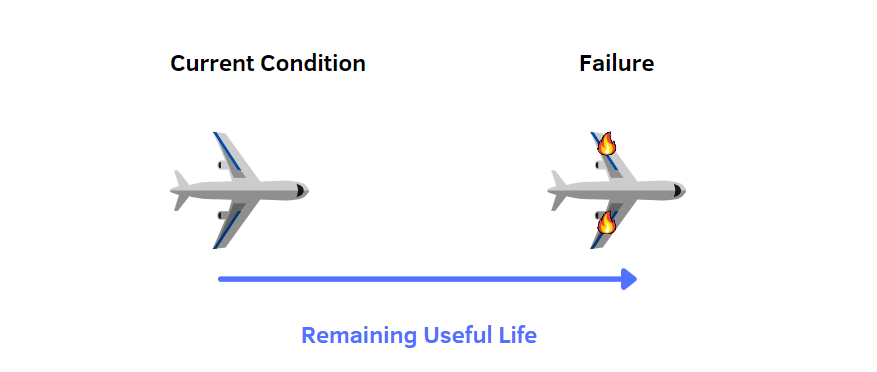
\includegraphics[scale=0.25]{airplane_diagram.png}

    \end{frame}

    \section{Prognostics and Health Management Society}
        \subsection{Organización}
            \begin{frame}
                \frametitle{Organización}
                \centering
                
\includegraphics[scale=0.3]{phm_logo.jpg}
                \begin{block}{Misión}
                    Sociedad que busca promover el desarrollo, crecimiento y reconocimiento del PHM como una rama de ingeniería a la vez que se avanza en la aplicación de PHM en la industria y la academia \cite{phm-mission}
                \end{block}
            \end{frame}

        \subsection{2021 PHM Conference Data Challenge}
            \begin{frame}
                \frametitle{2021 PHM Conference Data Challenge}
                \begin{block}{Objetivo}
                    Desarrollo de un modelo de predicción para el tiempo de vida útil restante de una turbina de avión comercial utilizando datos sintéticos del modelo CMAPSS \cite{arias2021aircraft}
                \end{block}

                \begin{itemize}
                    \item Lanzada en Agosto del 2021
                    \item Inclusión de datos de vuelos reales de aviones comerciales
                    \item Variaciones condiciones iniciales
                    \item 18 participantes, 3 ganadores
                \end{itemize}
            \end{frame}


    \section{Análisis de Datos}

        \subsection{Descripción de datos proporcionados}
        \begin{frame}
            \frametitle{Información general}
            \begin{table}[!htbp]
                \centering
                \scalebox{0.7}{
                \begin{tabular}{ |l|l|l|l|l|l| }
                    \hline
                    Archivo & Filas & Descriptores & Sensores & RUL & Auxiliares \\
                    \hline
                    N-CMAPSS\_DS01-005.h5 & 7,641,868 & 4 & 14 & 1 & 4 \\
                    N-CMAPSS\_DS02-006.h5 & 6,517,190 & 4 & 14 & 1 & 4 \\
                    N-CMAPSS\_DS03-012.h5 & 9,822,837 & 4 & 14 & 1 & 4 \\
                    N-CMAPSS\_DS04.h5 & 9,980,013 & 4 & 14 & 1 & 4 \\
                    N-CMAPSS\_DS05.h5 & 6,912,652 & 4 & 14 & 1 & 4 \\
                    N-CMAPSS\_DS06.h5 & 6,779,656 & 4 & 14 & 1 & 4 \\
                    N-CMAPSS\_DS07.h5 & 7,219,962 & 4 & 14 & 1 & 4 \\
                    N-CMAPSS\_DS08a-009.h5 & 8,608,386 & 4 & 14 & 1 & 4 \\
                    N-CMAPSS\_DS08c-008.h5 & 6,417,737 & 4 & 14 & 1 & 4 \\
                    \hline
                \end{tabular}}
                \label{tab:dataset_sizes}
                \caption{Tamaños de los conjuntos datos}
            \end{table}
            \begin{itemize}
                \item Archivo corrupto en base de datos
                \item Datos sintéticos del modelo CMAPSS
                \item Frecuencia de medición de 1 segundo
                \item Solamente se trabaja con datos de sensores y datos auxiliares \footnotemark
            \end{itemize}
            \footnotetext[1]{Los datos de los sensores virtuales no se encuentran en el conjunto de validación}
        \end{frame}

        \begin{frame}
            \frametitle{Datos proporcionados}
            \begin{table}[!htbp]
                \centering
                \scalebox{0.6}{
                \begin{tabular}{ |l|l|l| }
                    \hline
                    Symbol & Description & Units \\
                    \hline
                    alt & Altitude & ft \\
                    Mach & Flight Mach number & - \\
                    TRA & Throttle-resolver angle & \% \\
                    T2 & Total temperature at fan inlet & °R \\
                    \hline
                    Wf & Fuel flow & pps \\
                    Nf & Physical fan speed & rpm \\
                    Nc & Physical core speed & rpm \\
                    T24 & Total temperature at LPC outlet & °R \\
                    T30 & Total temperature at HPC outlet & °R \\
                    T48 & Total temperature at HPT outlet & °R \\
                    T50 & Total temperature at LPT outlet & °R \\
                    P15 & Total pressure in bypass-duct & psia \\
                    P21 & Total pressure at fan outlet & psia \\
                    P24 & Total pressure at LPC outlet & psia \\
                    Ps30 & Static pressure at HPC outlet & psia \\
                    P40 & Total pressure at burner outlet & psia \\
                    P50 & Total pressure at LPT outlet & psia \\
                    \hline
                    RUL & Remaining Useful Life & cycles \\
                    \hline
                    unit & Unit number & - \\
                    cycle & Flight cycle number & - \\
                    Fc & Flight class & - \\
                    hs & Health state & - \\
                    \hline
                \end{tabular}}
                \label{tab:dataset_info}
                \caption{Información general de los conjuntos de datos \cite{phm-conference}}
            \end{table}
        \end{frame}

        \subsection{Análisis Exploratorio de Datos}

        \begin{frame}
            \frametitle{Distribución de clases de vuelos}
            \begin{figure}[!htbp]
                \centering
                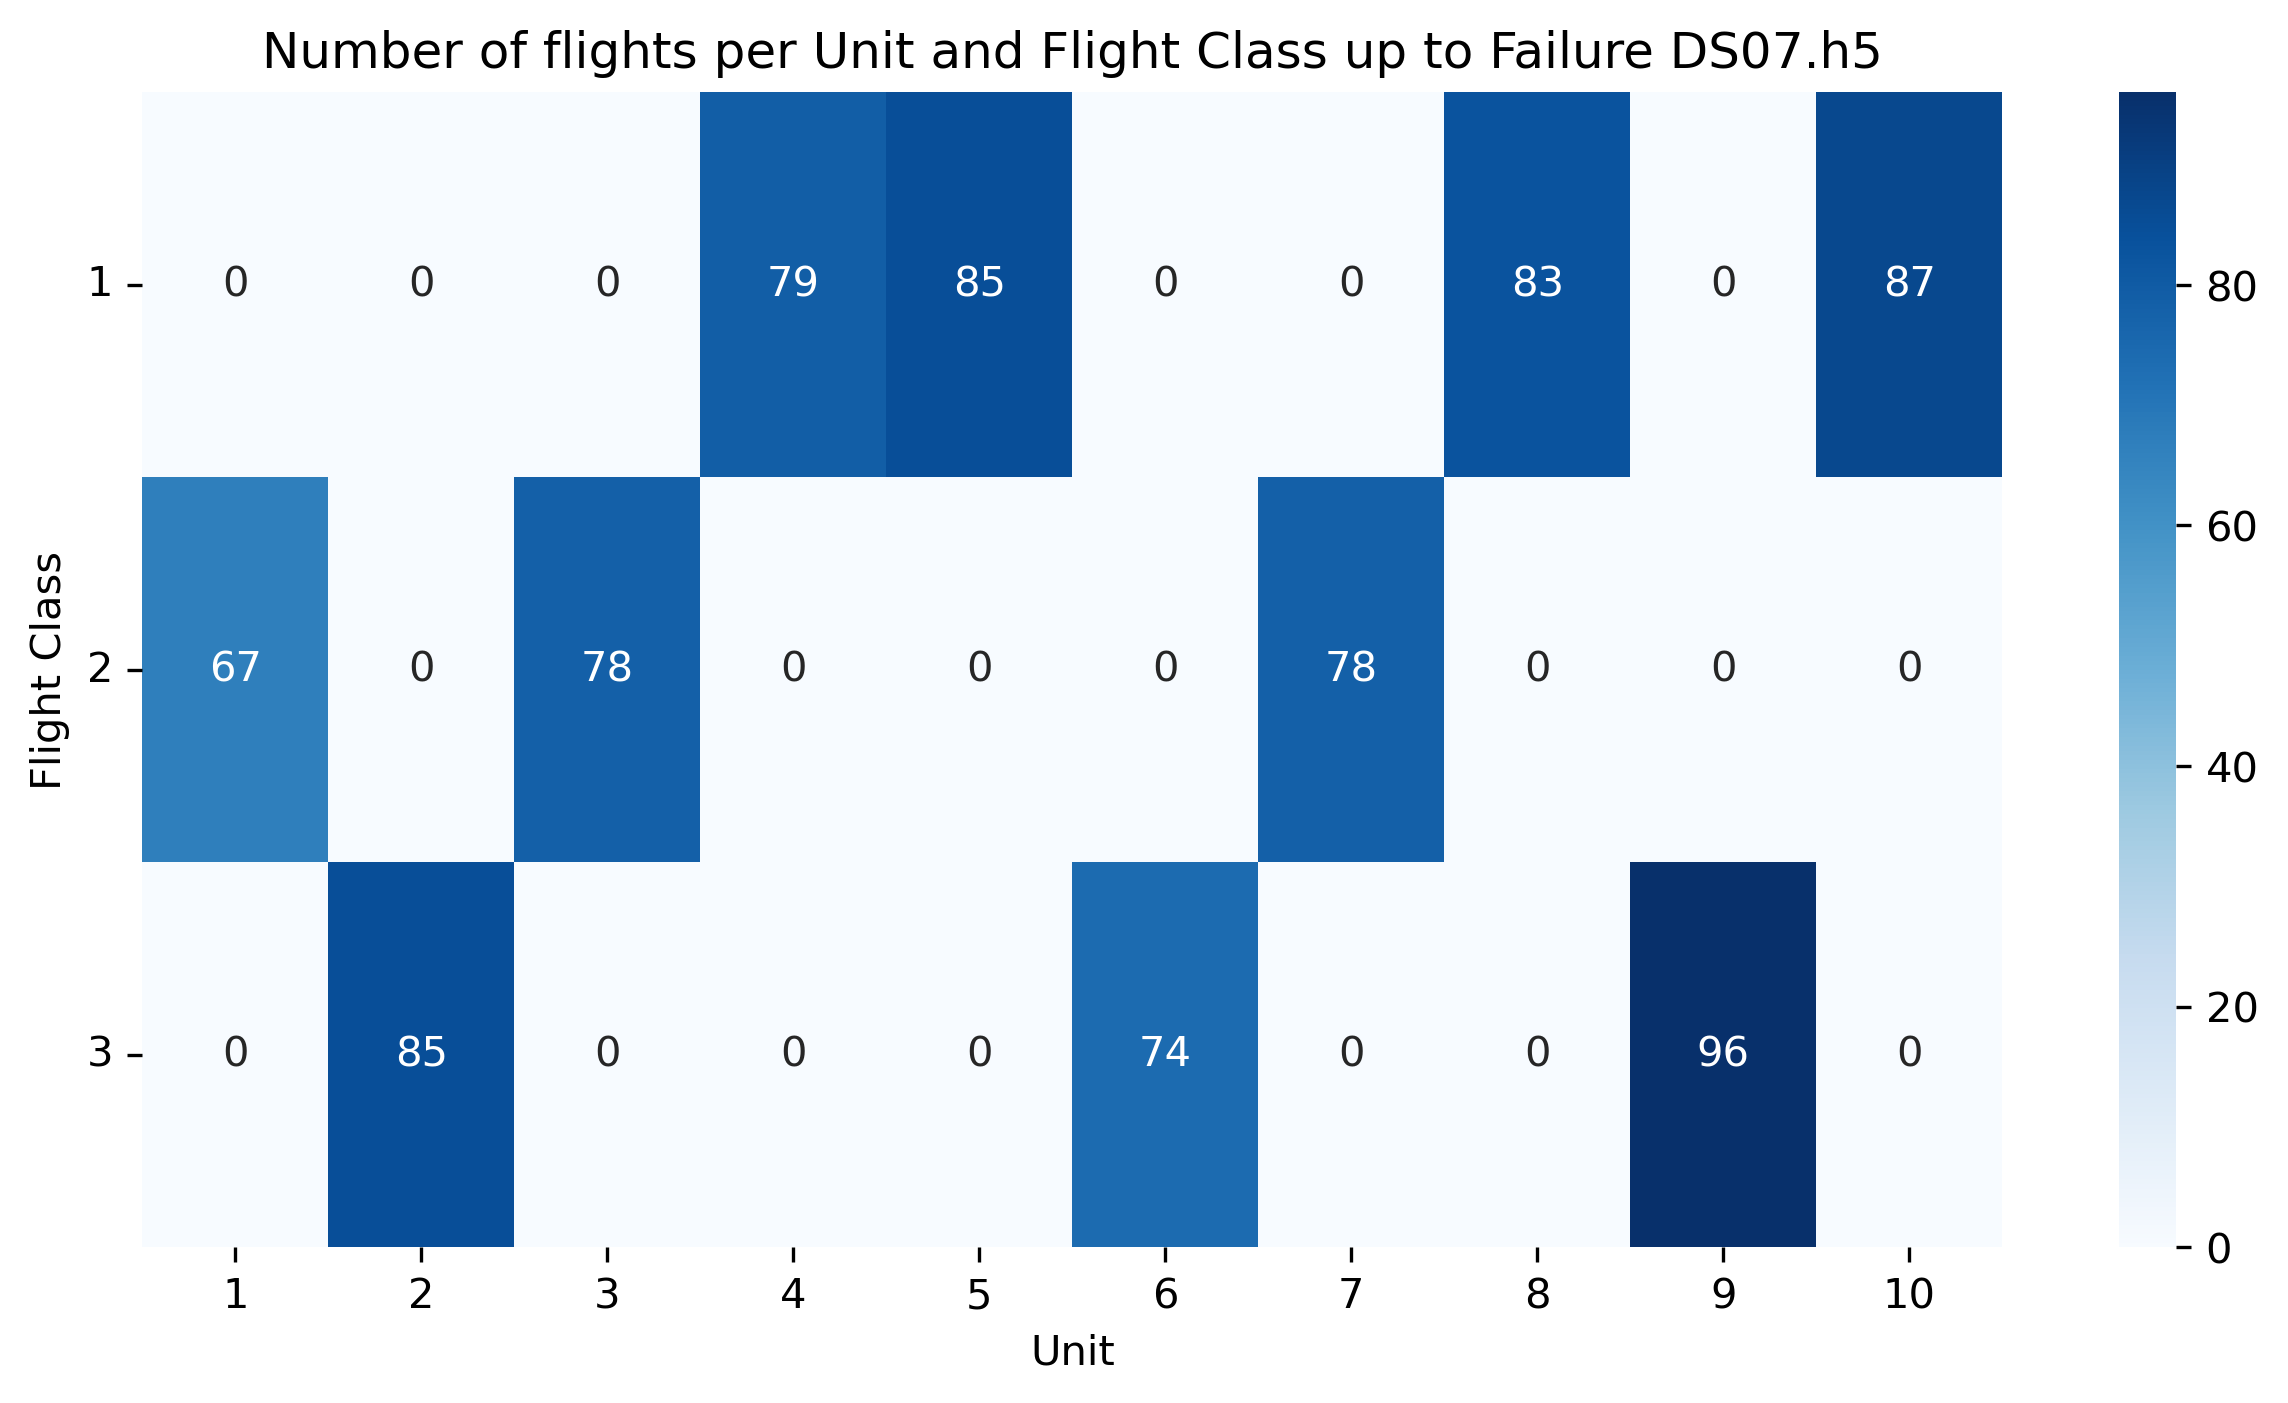
\includegraphics[scale=0.4]{fligt_class_per_unit_DS07.h5.png}
                \caption{Distribución de clases de vuelo}
            \end{figure}

            No hay aviones que participen en 2 tipos de vuelo en ningún momento
        \end{frame}

        \begin{frame}
            \frametitle{Perfil de vuelo}
            \begin{figure}[!htbp]
                \centering
                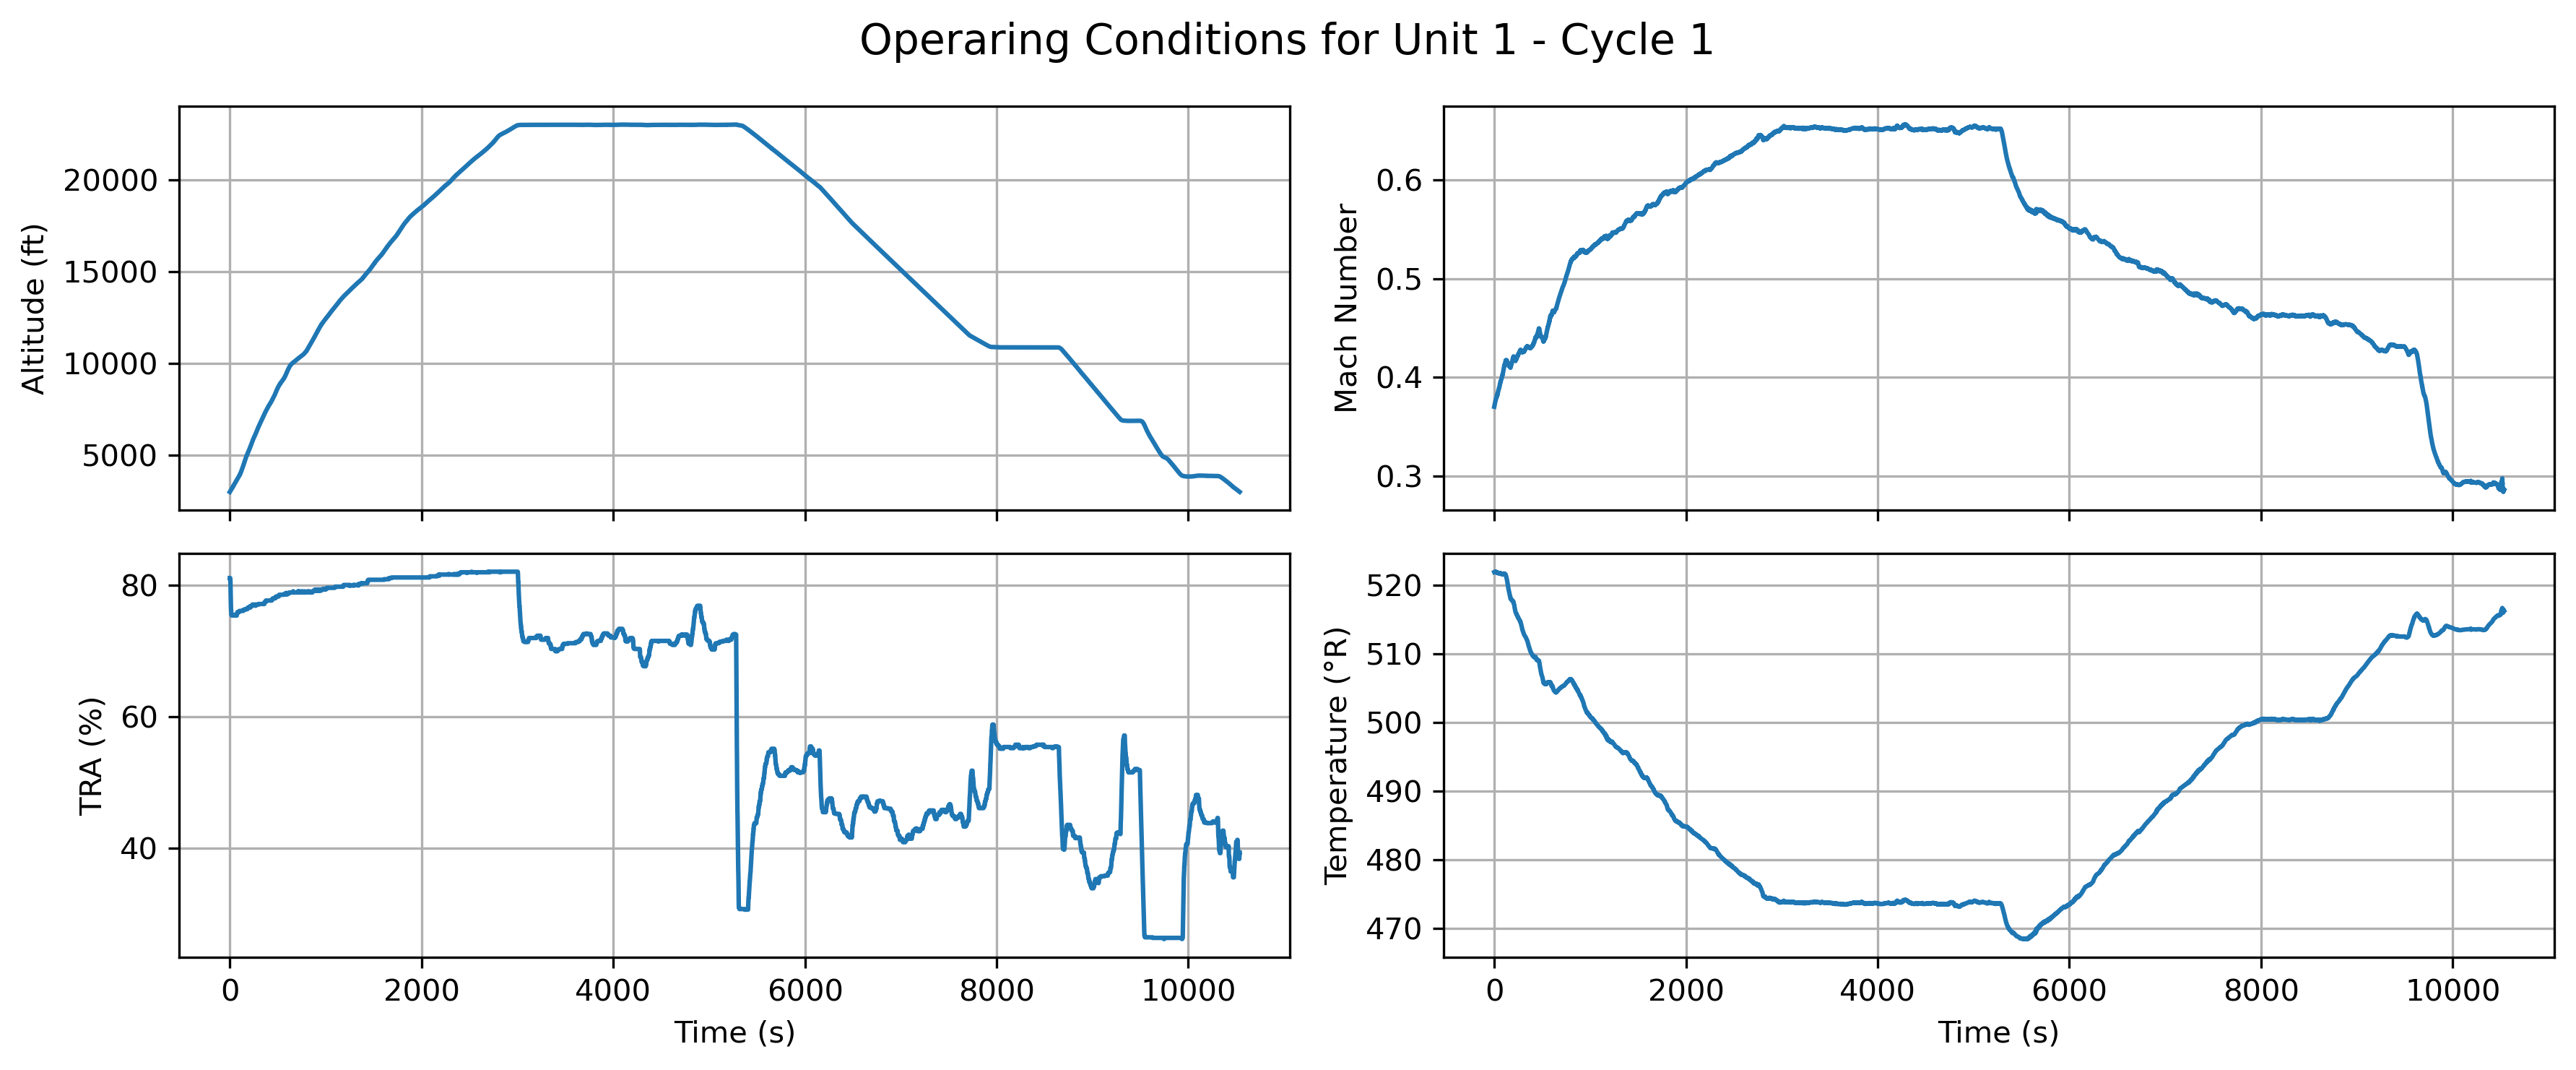
\includegraphics[scale=0.4]{operating_conditions_unit_1_cycle_1.png}
                \caption{Condiciones de vuelo para avión 1 en su primer vuelo}
            \end{figure}
        \end{frame}

        \begin{frame}
            \frametitle{Sumario de perfiles de vuelo}
            \begin{figure}[!htbp]
                \centering
                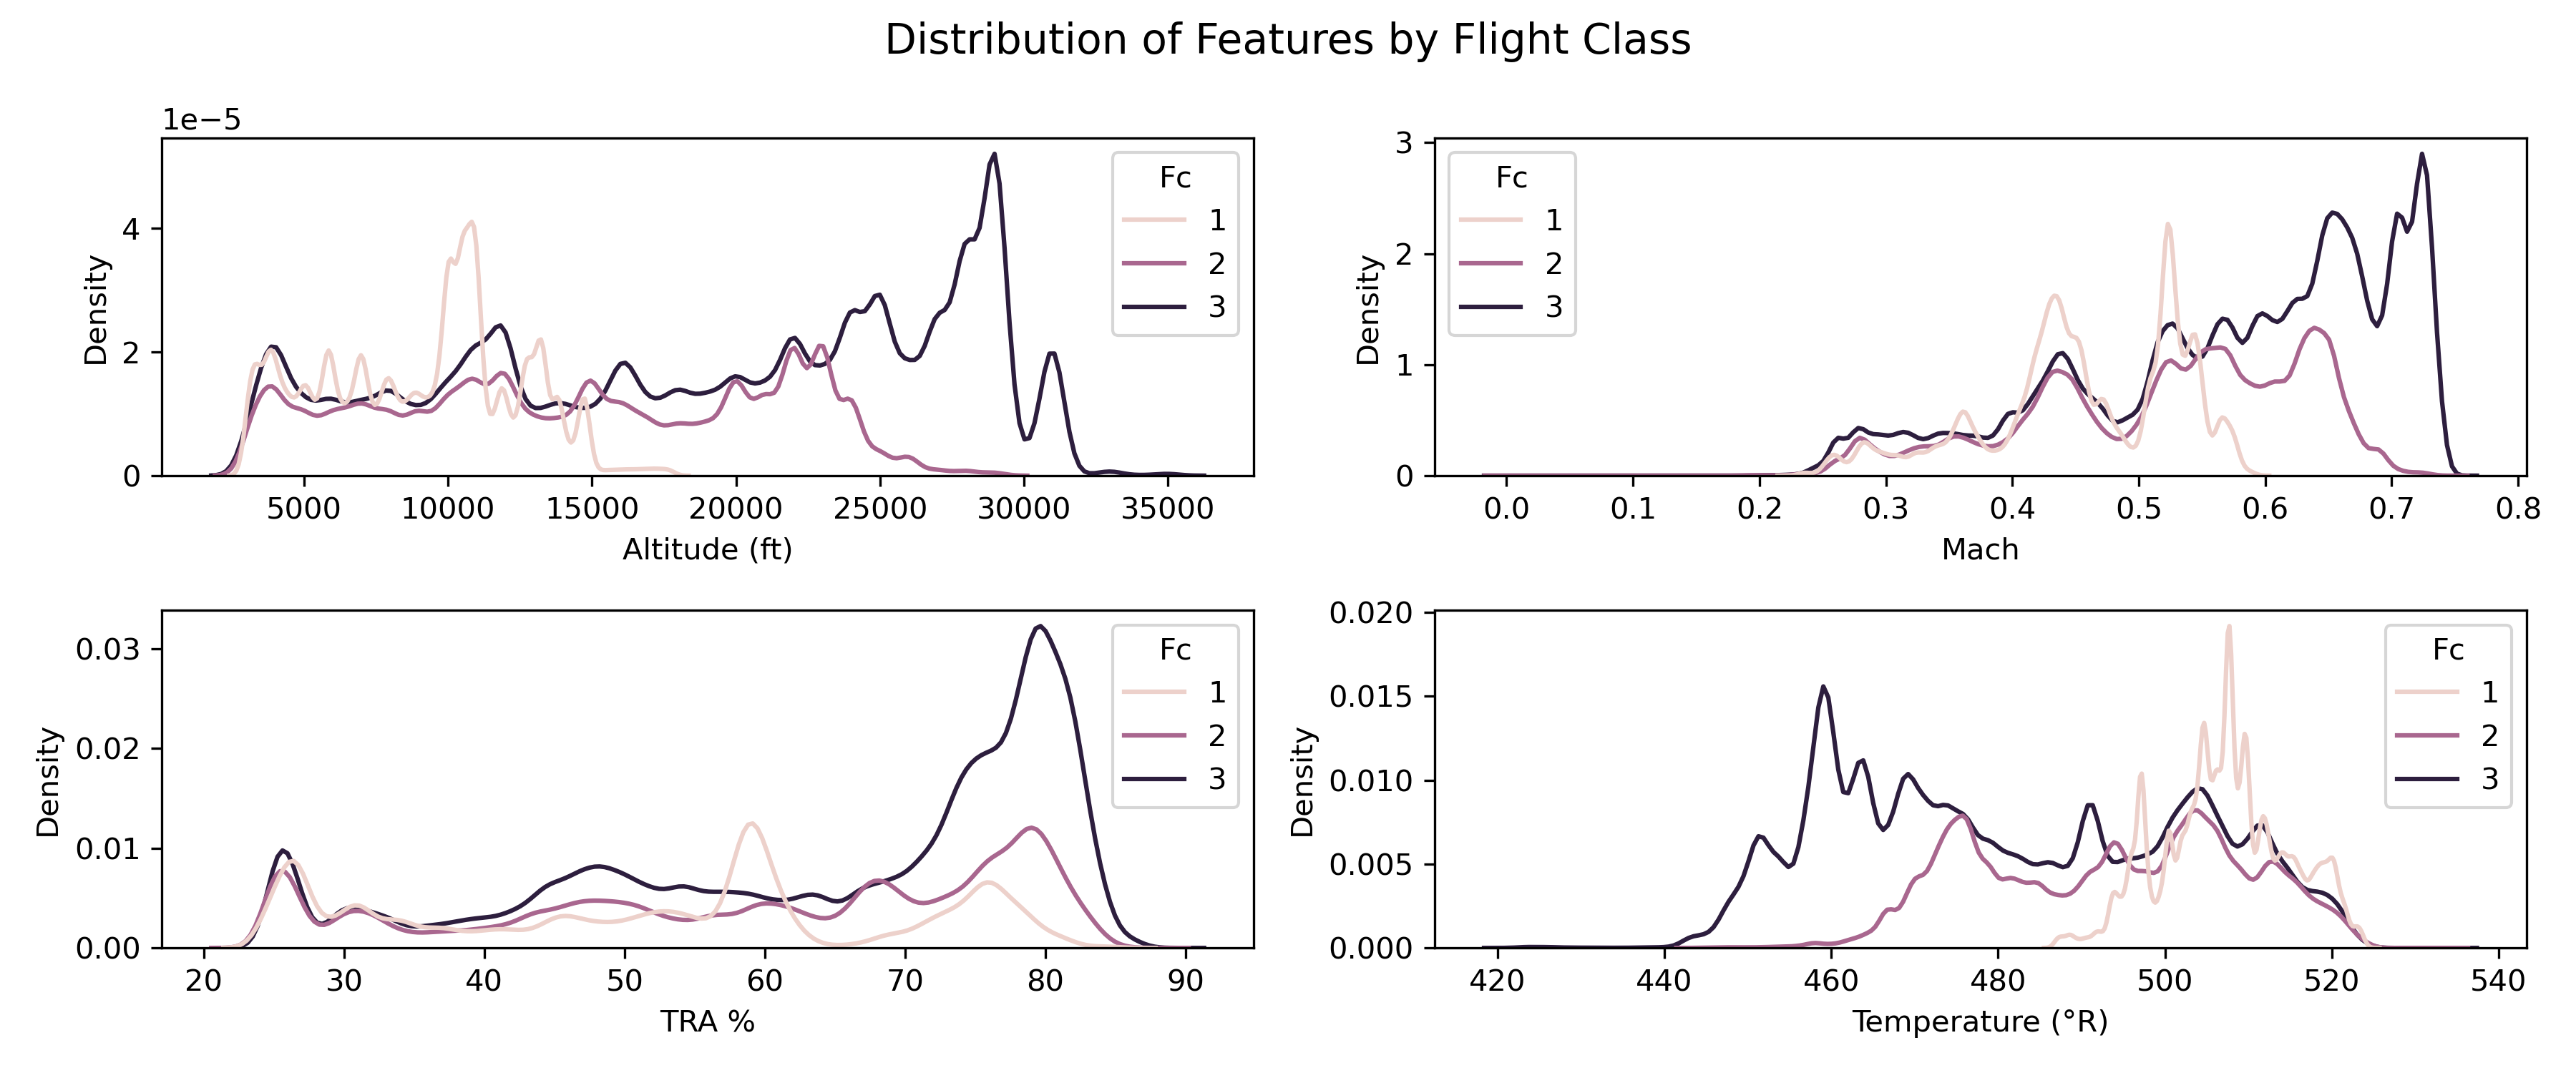
\includegraphics[scale=0.4]{features_per_condition_fc.png}
                \caption{Distribución de descriptores por clase de vuelo}
            \end{figure}
        \end{frame}

        \begin{frame}
            \frametitle{Ejemplo de medición de sensores}
            \begin{figure}[!htbp]
                \centering
                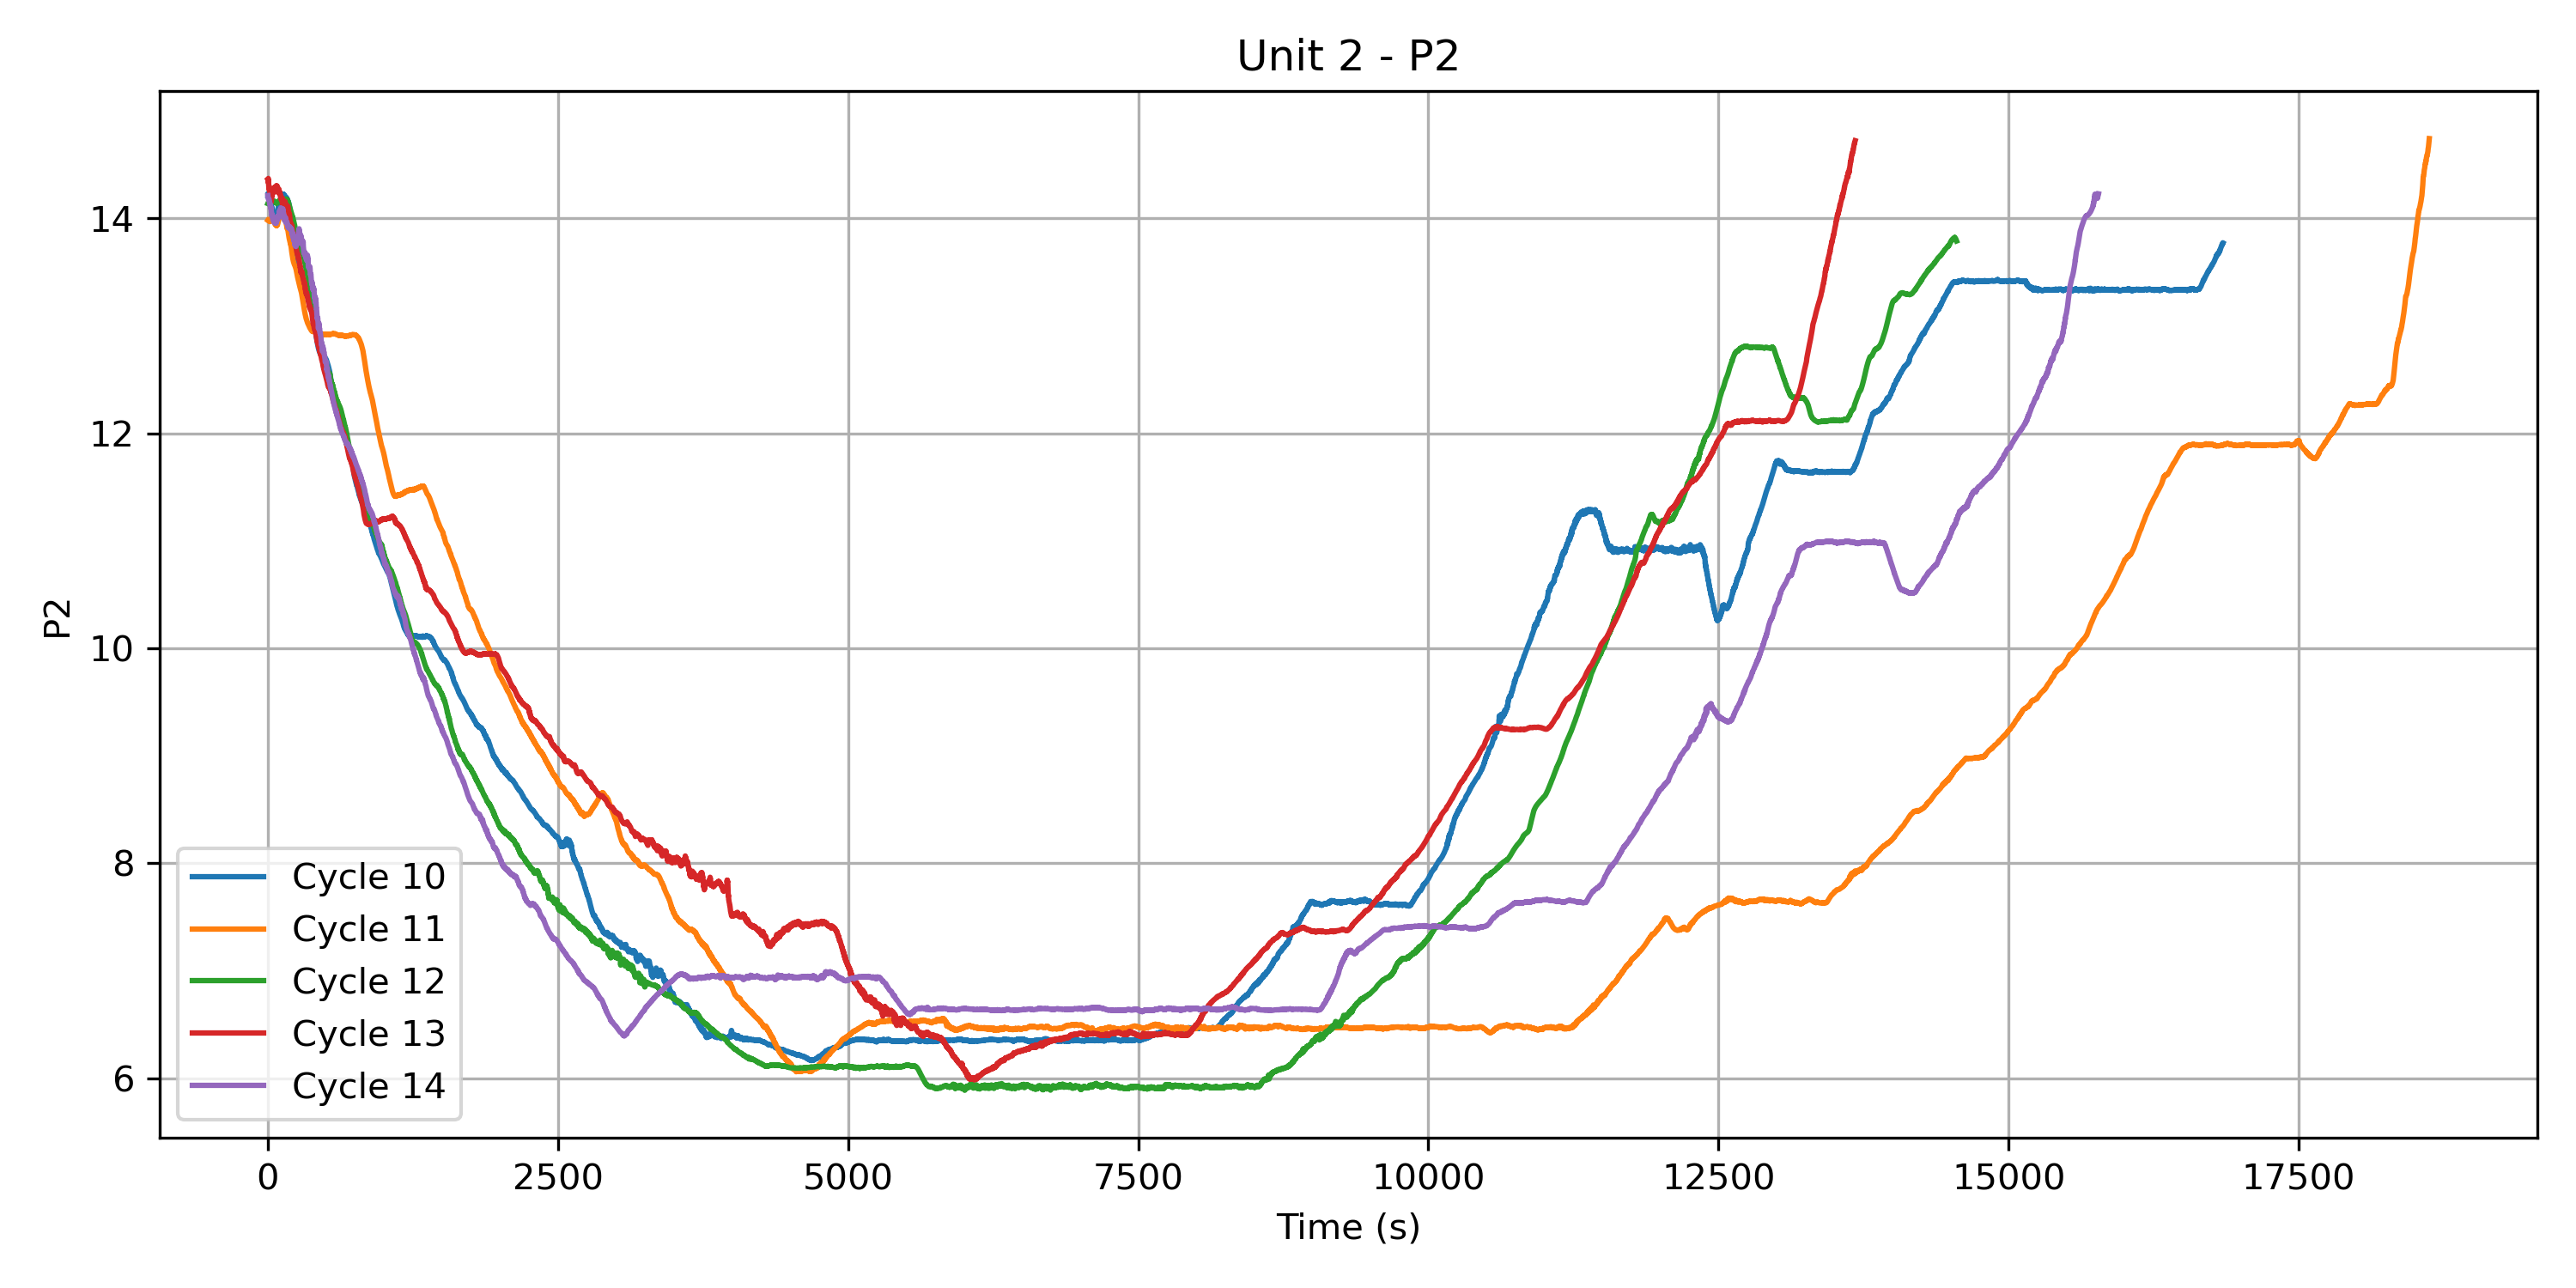
\includegraphics[scale=0.4]{unit_2_P2.png}
                \caption{Presión total/absoluta en la entrada del ventilador (psia)}
            \end{figure}
        \end{frame}

    \section{Comentarios, Mesa Redonda}

        \begin{frame}
            \frametitle{Comentarios, Mesa Redonda}
            \begin{itemize}
                \item Conjunto de datos fiel, no hay valores faltantes
                \item Es imposible cargar todos los datos de todos los archivos en memoria para un equipo convencional
                \item Variaciones considerables entre conjuntos de datos por modos de falla no presentes
            \end{itemize}
        \end{frame}


    \section{Referencias}
        \begin{frame}
            \frametitle{Referencias}
            \printbibliography
        \end{frame}

\end{document}